\part{Server}




\chapter{Overview}

首先,软件意义上的服务器就是一个管理资源并为用户提供服务的计算机软件,通常可以分为文件服务器(能使用户在其它计算机访问文件),数据库服务器和应用程序服务器(例如TCP服务器、UDP服务器、HTTP服务器、WebSocket服务器以及异步IO和Task服务器等)。


其次,运行服务器软件的计算机一般称为网络主机(host)\footnote{服务器与主机的意义可能不同,其中主机是通过终端给用户使用的,服务器是通过网络给客户端用户使用的。},可以通过网络对外提供服务。例如,可以通过Intranet对内网提供服务,也可以通过Internet对外提供服务。

Web服务器的定义有时会引起混淆,例如可以指用于网站的计算机,也可能是指Apache或Nginx等软件,而且运行Web服务器软件的计算机可以管理网页组件和回应网页浏览器的请求。

按照服务器软件工作在客户端-服务器还是浏览器-服务器模式,可以有很多形式的服务器,例如:

\begin{compactitem}
\item 文件服务器(File Server)或网络存储设备(Network Attached Storage),例如NetWare
\item 数据库服务器(Database Server),例如Oracle,MySQL,PostgreSQL,SQL Server等
\item 邮件服务器(Mail Server),例如Sendmail、Postfix、Qmail、Microsoft Exchange、Lotus Domino等
\item 网页服务器(Web Server),例如Apache、httpd和IIS等
\item FTP服务器(FTP Server),例如Pureftpd、Proftpd、WU-ftpd、Serv-U等
\item 域名服务器(DNS Server),例如Bind9等
\item 应用程序服务器(Application Server/AP Server),例如WebLogic、JBoss和GlassFish
\item 代理服务器(Proxy Server),例如Squid cache
\item NAT服务器,例如WINS(Windows Internet Name Service)服务器
\end{compactitem}


\clearpage
\section{Echo Server} 

\begin{figure}[htbp]
\centering
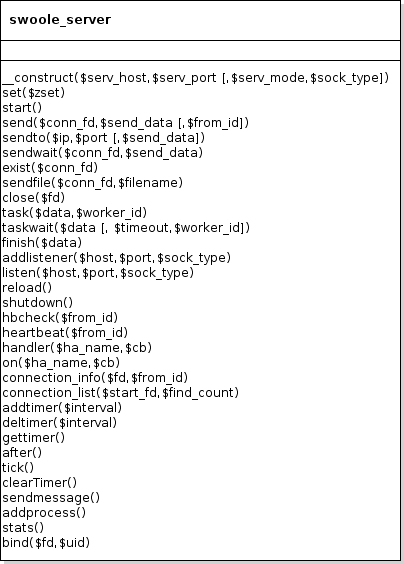
\includegraphics[scale=0.45]{class_swoole_server.png}
\caption{swoole\_server类}
\end{figure}


下面是一个基本的基于swoole的echo服务器实现,其中表示监听所有IP地址(包括 127.0.0.1、192.168.x.x 以及外网IP)。



\begin{lstlisting}[language=PHP]
<?php
// Server
class Server{
	private $serv;
	
	public function __construct(){
		$this->serv = new swoole_server("0.0.0.0",9501);
		$this->serv->set(array(
			'worker_num' => 8, // worker进程数
			'daemonize' => 0, // uint32_t, 是否守护进程化
			'max_request' => 10000, // worker进程的最大任务数
			'dispatch_mode' => 2, // 数据包分发策略,默认为2(固定模式)
			'debug_mode' => 1 // 无效参数,可以传入,不会执行
		));
		
		$this->serv->on('Start',array($this,'onStart'));
		$this->serv->on('Connect',array($this,'onConnect'));
		$this->serv->on('Receive',array($this,'onReceive'));
		$this->serv->on('Close',array($this,'onClose'));
		
		$this->serv->start();
	}
	// onStart回调在server运行前被调用
	public function onStart($serv){ 
		echo "Start\n";
	}
	// onConnect在有新客户端连接过来时被调用
	public function onConnect($serv,$fd,$from_id){ 
		$serv->send( $fd,"Hello {$fd}!" );
	}
	// onReceive函数在有数据发送到server时被调用
	public function onReceive(swoole_server $serv,$fd,$from_id,$data){
		echo "Get Message From Client {$fd}:{$data}\n";
	}
	// onClose在有客户端断开连接时被调用
	public function onClose($serv, $fd, $from_id){
		echo "Client {$fd} close connection\n";
	}
}

// 启动服务器
$server = new Server();
?>
\end{lstlisting}

创建一个swoole\_server基本分为如下三步:

\begin{compactitem}
\item 通过构造函数创建swoole\_server实例server;
\item 调用set函数设置swoole\_server实例的相关配置选项;
\item 调用on函数设置相关回调函数。
\end{compactitem}

这里,on方法的作用是注册swoole\_server的事件回调函数。

\begin{compactitem}
\item 在onStart处注册Start回调函数来启动swoole\_server实例server。
\item 在onConnect处注册Connect回调函数来让server监听新的连接。

如果有数据传入,则server可以调用send函数将处理结果发送出去。

\item 在onReceive处注册Receive回调函数来接收数据并处理。
\item 在onClose处注册Close回调函数处理客户端下线的事件。
\end{compactitem}

这里,需要注意的是启动swoole\_server实例之前,swoole\_server必须预先完成下面的操作:

\begin{compactitem}
\item 已创建了manager进程
\item 已创建了worker子进程
\item 已监听所有TCP/UDP端口
\item 已监听了定时器
\end{compactitem}

在完成上述操作后,swoole\_server的主Reactor开始接收事件,客户端可以connect到server。

onStart回调中仅允许echo、打印Log、修改进程名称,不得执行其他操作,而且onWorkerStart和onStart回调是在不同进程中并行执行的,不存在先后顺序。

在命令行中启动Echo Server的示例如下:

\begin{lstlisting}[language=PHP]
$ php server.php
Start
\end{lstlisting}

\section{Echo Client}

下面使用swoole\_client创建一个基于TCP的客户端实例,然后调用connect方法并指定同步还是模式来向指定的IP和端口发起连接请求。

\begin{compactitem}
\item 如果设置为1,则客户端使用同步阻塞模式(默认),recv和send操作都会产生网络阻塞。
\item 如果设置为0,则客户端使用异步传输模式,connect会立即返回true,但是实际上连接并未建立。
\end{compactitem}

在使用异步传输(即非阻塞socket)时,send/recv执行前必须使用swoole\_client\_select来检测是否完成了连接。

无论使用同步还是异步模式来进行数据传输,在连接成功后才可以通过recv()和send()方法来接收和发送请求。



\begin{lstlisting}[language=PHP]
<?php
// Client
class Client{
	private $client;
	
	public function __construct(){
		// 创建tcp socket
		$this->client = new swoole_client(SWOOLE_SOCK_TCP);
	}
	
	public function connect(){
		if(!$this->client->connect("127.0.0.1",9501,1)){
			echo "Error: {$fp->errMsg}[{$fp->errCode}]\n";
		}
		$message = $this->client->recv();
		echo "Get Message From Server: {$message}\n";
		
		fwrite(STDOUT,"请输入消息: ");
		$msg = trim(fgets(STDIN));
		$this->client->send($msg);
	}
}
$client = new Client();
$client->connect();
?>
\end{lstlisting}


在使用非阻塞socket时,不能在connect后使用send/recv,通过isConnected()判断也是false。只有当连接成功后,系统会自动回调onConnect,这时才可以使用send/recv。

在命令行中运行echo client的代码如下:



\begin{lstlisting}[language=PHP]
$ php client.php
Get Message From Server: Hello 1!
请输入消息:
\end{lstlisting}




\begin{lstlisting}[language=PHP]

\end{lstlisting}




\begin{lstlisting}[language=PHP]

\end{lstlisting}




\begin{lstlisting}[language=PHP]

\end{lstlisting}




\begin{lstlisting}[language=PHP]

\end{lstlisting}






\chapter{TCP}


\section{Overview}



 TCP是一种面向连接的、可靠的、基于字节流的传输层通信协议,在简化的计算机网络OSI模型中完成第四层传输层所指定的功能,用户数据报协议(UDP)则是同一层内另一个重要的传输协议。
 
 在因特网协议族(Internet protocol suite)中,TCP层是位于IP层之上,应用层之下的中间层。不同主机的应用层之间经常需要可靠的、像渠道一样的连接,但是IP层不提供这样的流机制,而是提供不可靠的包交换。

应用层向TCP层发送用于网间传输的、用8位字节表示的数据流,然后TCP把数据流分区成适当长度的报文段(通常受该计算机连接的网络的数据链路层的最大传输单元(MTU)的限制)。之后TCP把结果包传给IP层,由它来通过网络将包传送给接收端实体的TCP层。

TCP为了保证不发生丢包,就给每个包一个序号,同时序号也保证了传送到接收端实体的包的按序接收。

接收端实体对已成功收到的包发回一个相应的确认(ACK),如果发送端实体在合理的往返时延(RTT)内未收到确认,那么对应的数据包就被假设为已丢失将会被进行重传。

TCP用一个校验和函数来检验数据是否有错误,而且在发送和接收时都要计算校验和。

TCP连接包括三个状态:连接创建、数据传送和连接终止,操作系统将 TCP 连接抽象为套接字的编程接口给程序使用,因此要经历一系列的状态改变。

TCP使用了端口号(Port number)的概念来标识发送方和接收方的应用层,可能的和被正式承认的端口号有65535($2^{16}-1$)个。


对每个TCP连接的一端都有一个相关的16位的无符号端口号分配给它们,端口可以被分为三类:众所周知的、注册的和动态/私有的。

\begin{compactitem}
\item 众所周知的端口号是由因特网赋号管理局(IANA)来分配的,并且通常被用于系统一级或根进程。

众所周知的应用程序作为服务器程序来运行,并被动地侦听经常使用这些端口的连接。例如FTP、TELNET、SMTP、HTTP等。

\item 注册的端口号通常被用来作为终端用户连接服务器时短暂地使用的源端口号,但它们也可以用来标识已被第三方注册了的、被命名的服务。

\item 动态/私有的端口号在任何特定的TCP连接外不具有任何意义。

\end{compactitem}


注意,TCP并不是对所有的应用都适合,一些新的带有一些内在的脆弱性的运输层协议也被设计出来。比如,实时应用并不需要甚至无法忍受TCP的可靠传输机制。

在实时类型的应用(例如视频通话等)中,通常允许一些丢包、出错或拥塞,而不是去校正它们,因此在实时流多媒体(如因特网广播)、实时多媒体播放器和游戏、IP电话(VoIP)中可以不使用TCP。

任何不是很需要可靠性或者是想将功能减到最少的应用可以避免使用TCP,因此在很多情况下,当只需要多路复用应用服务时,用户数据报协议(UDP)可以代替TCP为应用提供服务。


\subsection{Establishment}


TCP用三路握手(three-way handshake)过程创建一个连接。在连接创建过程中,很多参数要被初始化,例如序号被初始化以保证按序传输和连接的强壮性。

一对终端同时初始化一个它们之间的连接是可能的。但通常是由一端打开一个套接字(socket)然后监听来自另一方的连接,这就是通常所指的被动打开(passive open)。服务器端被被动打开以后,用户端就能开始创建主动打开(active open)。

\begin{compactenum}
\item 客户端通过向服务器端发送一个SYN来创建一个主动打开,作为三路握手的一部分。客户端把这段连接的序号设定为随机数 A。
\item 服务器端应当为一个合法的SYN回送一个SYN/ACK。ACK 的确认码应为 A+1,SYN/ACK 包本身又有一个随机序号 B。
\item 最后,客户端再发送一个ACK。当服务端受到这个ACK的时候,就完成了三路握手,并进入了连接创建状态。此时包序号被设定为收到的确认号 A+1,而响应则为 B+1。
\end{compactenum}

\begin{figure}[htbp]
\centering
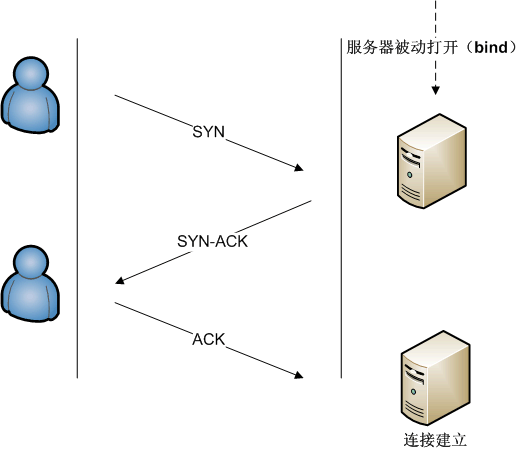
\includegraphics[scale=0.5]{Connection_TCP.png}
\caption{TCP连接的正常创建}
\end{figure}



\subsection{Transmission}

在TCP的数据传送状态,很多重要的机制保证了TCP的可靠性和强壮性,其中包括:

\begin{compactitem}
\item 使用序号,对收到的TCP报文段进行排序以及检测重复的数据;
\item 使用校验和来检测报文段的错误;
\item 使用确认和计时器来检测和纠正丢包或延时。
\end{compactitem}

在TCP的连接创建状态,两个主机的TCP层间要交换初始序号(ISN,Initial Sequence Number),而且这些序号用于标识字节流中的数据,并且还是对应用层的数据字节进行记数的整数。

通常情况下,在每个TCP报文段中都有一对序号和确认号,TCP报文发送者认为自己的字节编号为序号,而认为接收者的字节编号为确认号。

TCP报文的接收者为了确保可靠性,在接收到一定数量的连续字节流后才发送确认,其实这是对TCP的一种扩展,通常称为选择确认(Selective Acknowledgement),通过选择确认使得TCP接收者可以对乱序到达的数据块进行确认,而且每一个字节传输过后,ISN号都会递增1。


通过使用序号和确认号,TCP层可以把收到的报文段中的字节按正确的顺序交付给应用层。

序号是32位的无符号数,在它增大到$2^{32}-1$时,便会回绕到0,因此可以确保TCP中关键的一个操作——ISN的选择的强壮性和安全性。

\begin{compactenum}
\item 发送方首先发送第一个包含序列号为1(可变化)和1460字节数据的TCP报文段给接收方。接收方以一个没有数据的TCP报文段来回复(只含报头),用确认号1461来表示已完全收到并请求下一个报文段。

\item 发送方然后发送第二个包含序列号为1461和1460字节数据的TCP报文段给接收方。正常情况下,接收方以一个没有数据的TCP报文段来回复,用确认号2921(1461+1460)来表示已完全收到并请求下一个报文段。发送接收这样继续下去。

\item 然而当这些数据包都是相连的情况下,接收方没有必要每一次都回应。比如,他收到第1到5条TCP报文段,只需回应第五条就行了。在例子中第3条TCP报文段被丢失了,所以尽管他收到了第4和5条,然而他只能回应第2条。

\item 发送方在发送了第三条以后,没能收到回应,因此当定时器(timer)到期(expire)时,他重发第三条。(每次发送者发送一条TCP报文段后,都会再次启动一次时钟:RTT)。

\item 这次第三条被成功接收,接收方可以直接确认第5条,因为4,5两条已收到。

\end{compactenum}

\begin{figure}[htbp]
\centering
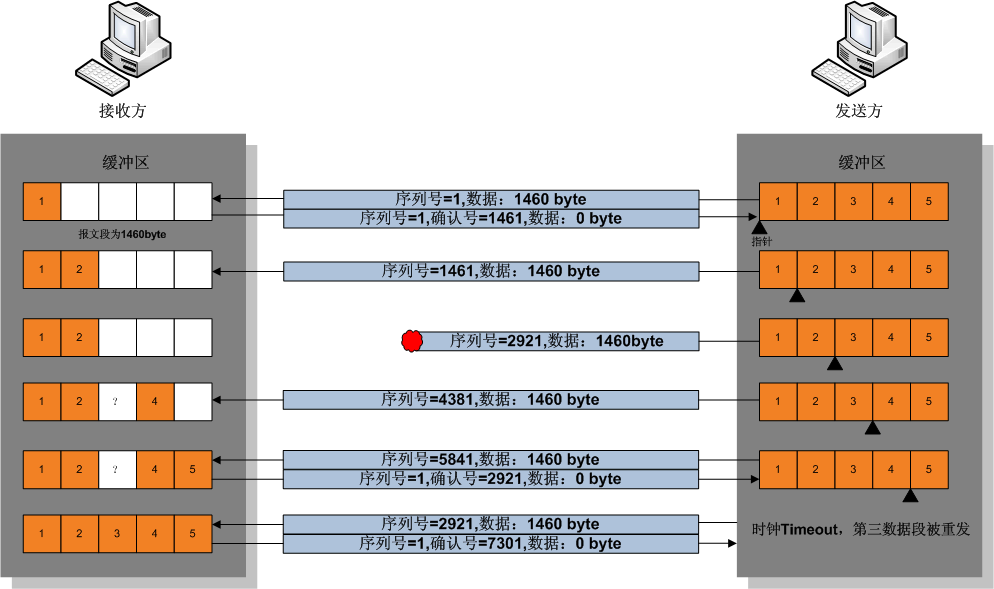
\includegraphics[scale=0.5]{Tcp_transport_example.png}
\caption{TCP数据传输}
\end{figure}

TCP的16位的校验和(checksum)的计算和检验过程如下:

发送者将TCP报文段的头部和数据部分的和计算出来,再对其求反码(一的补数),就得到了校验和,然后将结果装入报文中传输。

这里,用反码和的原因是这种方法的循环进位使校验和可以在16位、32位、64位等情况下的计算结果再叠加后相同。

接收者在收到报文后再按相同的算法计算一次校验和。这里使用的反码使得接收者不用再将校验和字段保存起来后清零,而可以直接将报文段连同校验加总。如果计算结果是全部为一,那么就表示了报文的完整性和正确性。

TCP校验和也包括了96位的伪头部,其中有源地址、目的地址、协议以及TCP的长度,从而可以避免报文被错误地路由。

按照现在的标准,TCP的校验和是一个比较脆弱的校验。出错概率高的数据链路层需要更高的能力来探测和纠正连接错误。

如果在今天重新设计TCP,很可能使用一个32位的CRC校验来纠错,而不是使用校验和。但是通过在第二层使用通常的CRC校验或更完全一点的校验可以部分地弥补这种脆弱的校验。

第二层是在TCP层和IP层之下的(比如PPP或以太网)使用了这些校验,但是这也并不意味着TCP的16位校验和是冗余的。

根据对因特网传输的观察,表明在受CRC校验保护的各跳之间,软件和硬件的错误通常也会在报文中引入错误,而端到端的TCP校验能够捕捉到很多的这种错误,这就是应用中的端到端原则。

流量控制可以避免主机分组发送得过快而使接收方来不及完全收下,因此TCP和UDP的主要不同在于:

\begin{compactitem}
\item 有序数据传输
\item 重发丢失的数据包
\item 舍弃重复的数据包
\item 无错误数据传输
\item 阻塞/流量控制
\item 面向连接(确认有创建三方交握,连接已创建才作传输)
\end{compactitem}

\subsection{Termination}

连接终止使用了四路握手过程(four-way handshake),在这个过程中每个终端的连接都能独立地被终止,因此一个典型的拆接过程需要每个终端都提供一对FIN和ACK。

\begin{figure}[htbp]
\centering
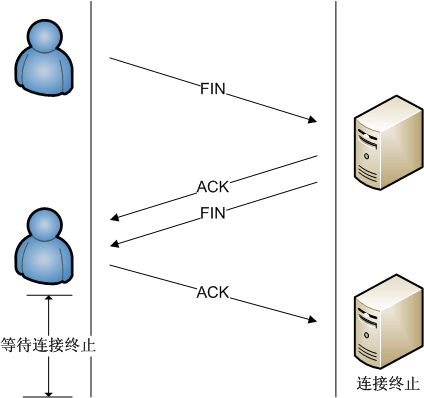
\includegraphics[scale=0.5]{Deconnection_TCP.png}
\caption{TCP连接的正常终止}
\end{figure}


\section{State Diagram}

下表为 TCP 状态码列表,以 S 指代服务器,C 指代客户端,S\&C 表示两者,S/C 表示两者之一:

\begin{figure}[htbp]
\centering
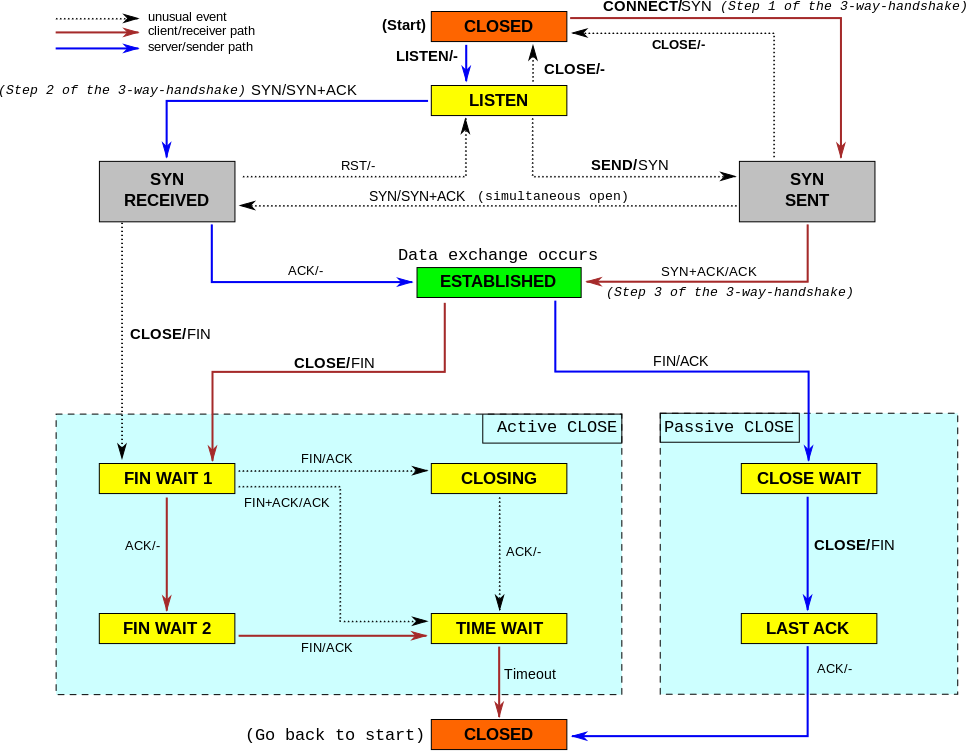
\includegraphics[scale=0.5]{Tcp_state_diagram.png}
\caption{TCP 状态码列表}
\end{figure}

\zihao{6}
\begin{longtable}{|m{70pt}|m{100pt}|m{250pt}|}
%head
\multicolumn{3}{r}{}
\tabularnewline\hline
状态码&状态&描述
\endhead
%endhead

%firsthead
\caption{TCP 状态码列表}\\
\hline
状态码&状态&描述
\endfirsthead
%endfirsthead

%foot
\multicolumn{3}{r}{}
\endfoot
%endfoot

%lastfoot
\endlastfoot
%endlastfoot

\hline
LISTEN S&侦听状态 & 等待从任意远程 TCP 端口的连接请求。\\
\hline
SYN-SENT C& 在发送连接请求后等待匹配的连接请求。&通过connect()函数向服务器发出一个同步(SYNC)信号后进入此状态。\\
\hline
SYN-RECEIVED S &  & 已经收到并发送同步(SYNC)信号之后等待确认(ACK)请求。\\
\hline
ESTABLISHED S\&C & 连接已经打开,收到的数据可以发送给用户。&数据传输步骤的正常情况。此时连接两端是平等的。\\
\hline
FIN-WAIT-1 S\&C &  & 主动关闭端调用close()函数发出FIN请求包,表示本方的数据发送全部结束,等待TCP连接另一端的确认包或FIN请求包。\\
\hline
FIN-WAIT-2 S\&C & &主动关闭端在FIN-WAIT-1状态下收到确认包,进入等待远程 TCP 的连接终止请求的半关闭状态。这时可以接收数据,但不再发送数据。\\
\hline
CLOSE-WAIT S\&C & &被动关闭端接到FIN后,就发出ACK以回应FIN请求,并进入等待本地用户的连接终止请求的半关闭状态。这时可以发送数据,但不再接收数据。\\
\hline
CLOSING S\&C & & 在发出FIN后,又收到对方发来的FIN后,进入等待对方对连接终止(FIN)的确认(ACK)的状态。\\
\hline
LAST-ACK S\&C & & 被动关闭端全部数据发送完成之后,向主动关闭端发送FIN,进入等待确认包的状态。\\
\hline
TIME-WAIT S/C &  & 主动关闭端接收到FIN后,就发送ACK包,等待足够时间\footnote{按照 RFC 793,一个连接可以在 TIME-WAIT 保证最大四分钟,即最大分段寿命(maximum segment lifetime)的2倍。}以确保被动关闭端收到了终止请求的确认包。\\
\hline
CLOSED S\&C & & 完全没有连接。\\
\hline
\end{longtable}
\zihao{5}

\clearpage

\section{TCP Server}


下面的示例创建一个TCP服务器,监听本机9501端口,当客户端Socket通过网络发送一个 hello 字符串时,服务器会回复一个 Swoole TCP Server: hello 字符串。


\begin{lstlisting}[language=PHP]
//创建swoole_server对象,在127.0.0.1监听9501端口
$serv = new swoole_server("127.0.0.1", 9501);

$serv->set(array(
    'worker_num' => 8,   //工作进程数量
    'daemonize' => 0 //是否作为守护进程
));

// 监听连接进入事件
$serv->on('connect', function ($serv, $fd){
    echo "Client:Connect.\n";
});

//监听数据发送事件
$serv->on('receive', function ($serv, $fd, $from_id, $data) {
    $serv->send($fd, 'Swoole TCP Server: '.$data);
    $serv->close($fd);
});

//监听连接关闭事件
$serv->on('close', function ($serv, $fd) {
    echo "Client: Close.\n";
});

//启动服务器
$serv->start();
\end{lstlisting}

swoole\_server是异步服务器,所以是通过监听事件的方式来编写程序的。

当对应的事件发生时底层会主动回调指定的PHP函数,例如当有新的TCP连接进入时会执行onConnect事件回调,当某个连接向服务器发送数据时会回调onReceive函数。

\begin{compactitem}
\item 服务器可以同时被成千上万个客户端连接,\texttt{\$fd}就是客户端连接的唯一标识符
\item 调用 \texttt{\$server->send()}方法向客户端连接发送数据,参数就是\texttt{\$fd}客户端标识符
\item 调用 \texttt{\$server->close()}方法可以强制关闭某个客户端连接
\item 客户端可能会主动断开连接,此时会触发onClose事件回调
\end{compactitem}

在命令行下运行server.php程序来启动Swoole TCP Server,如果启动成功后可以使用 netstat 工具看到,已经在监听9501端口,然后就可以使用telnet/netcat工具连接服务器。

\begin{lstlisting}[language=PHP]
$ php tcp_server.php 
\end{lstlisting}


\begin{compactitem}
\item 在本机使用telnet/netcat连接Swoole TCP Server:

\begin{lstlisting}[language=PHP]
$ telnet 127.0.0.1 9501
Trying 127.0.0.1...
Connected to 127.0.0.1.
Escape character is '^]'.
hello
Swoole TCP Server: hello
\end{lstlisting}

\item 在远程主机使用telnet/netcat连接Swoole TCP Server:

\begin{lstlisting}[language=PHP]
$ telnet 121.40.126.146 9501
Trying 121.40.126.146...
telnet: connect to address 121.40.126.146: Connection refused
\end{lstlisting}

\end{compactitem}




\begin{lstlisting}[language=PHP]

\end{lstlisting}




\begin{lstlisting}[language=PHP]

\end{lstlisting}




\begin{lstlisting}[language=PHP]

\end{lstlisting}







\section{TCP Client}

除了使用telnet/netcat来连接Swoole TCP Server之外,也可以自己实现TCP Client来进行连接和通信。


\begin{lstlisting}[language=PHP]
$client = new swoole_client(SWOOLE_SOCK_TCP, SWOOLE_SOCK_ASYNC);
//设置事件回调函数
$client->on("connect", function($cli) {
    $cli->send("hello world\n");
});
$client->on("receive", function($cli, $data){
    echo "Received: ".$data."\n";
});
$client->on("error", function($cli){
    echo "Connect failed\n";
});
$client->on("close", function($cli){
    echo "Connection close\n";
});
//发起网络连接
//$client->connect('127.0.0.1', 9501, 0.5);
$client->connect('121.40.126.146', 9501, 0.5);
\end{lstlisting}

\begin{compactitem}
\item SWOOLE\_SOCK\_TCP 创建tcp socket
\item SWOOLE\_SOCK\_TCP6 创建tcp ipv6 socket
\item SWOOLE\_SOCK\_UDP 创建udp socket
\item SWOOLE\_SOCK\_UDP6 创建udp ipv6 socket
\item SWOOLE\_SOCK\_SYNC 同步客户端
\item SWOOLE\_SOCK\_ASYNC 异步客户端
\end{compactitem}



在远程服务器上开启Server TCP Server:

\begin{lstlisting}[language=PHP]
$ php tcp_server.php
\end{lstlisting}

在本地计算机上执行Swoole TCP Client:

\begin{lstlisting}[language=PHP]
$ php tcp_client.php
Received: Swoole TCP Server: hello world

Connection close
\end{lstlisting}

实际上,\texttt{hello world}从远程服务器上发回,因此如果远程服务器关闭,那么就可能返回如下的错误:

\begin{lstlisting}[language=PHP]
$ php tcp_client.php
Unknown: connect to server [121.40.126.146:9501] failed. 
Error: Connection refused [111]. in Unknown on line 0

Warning: Unknown: connect to server [121.40.126.146:9501] failed. 
Error: Connection refused [111]. in Unknown on line 0

Connect failed
\end{lstlisting}

正常情况下,远程服务器上的Swoole TCP Server会产生如下的输出:


\begin{lstlisting}[language=PHP]
$ php tcp_server.php 
Client:Connect.
Client: Close.
\end{lstlisting}


\chapter{UDP}


\section{Overview}

UDP(User Datagram Protocol,用户数据报协议)是一个简单的面向数据报的传输层协议,其正式规范为 RFC 768。

在TCP/IP模型中,UDP为网络层以上和应用层以下提供了一个简单的接口。

UDP只提供数据的不可靠传递,它一旦把应用程序发给网络层的数据发送出去,就不保留数据备份,所以UDP有时候也被认为是不可靠的数据报协议,而且UDP在IP数据报的头部仅仅加入了复用和数据校验(字段)。

UDP首部字段由4个部分组成,其中两个是可选的,其中分别都是16bit的来源端口和目的端口用来标记发送和接受的应用进程。

UDP不需要应答,所以来源端口是可选的,如果来源端口不用,那么置为零。在目的端口后面是长度固定的以字节为单位的长度域,用来指定UDP数据报包括数据部分的长度,长度最小值为8byte。

首部剩下的16bit是用来对首部和数据部分一起做校验和(Checksum)的,这部分是可选的,但是在实际应用中一般都使用这一功能。

由于缺乏可靠性且属于非连接导向协定,UDP应用一般必须允许一定量的丢包、出错和复制贴上,但是有些应用(比如TFTP),如果需要则必须在应用层增加根本的可靠机制。

绝大多数UDP应用都不需要可靠机制,甚至可能因为引入可靠机制而降低性能,因此流媒体(串流技术)、即时多媒体游戏和IP电话(VoIP)一定是典型的UDP应用。如果某个应用需要很高的可靠性,那么可以用TCP来代替UDP。

由于缺乏拥塞控制(congestion control),需要基于网络的机制来减少因失控和高速UDP流量负荷而导致的拥塞崩溃效应。换句话说,因为UDP发送者不能够检测拥塞,所以像使用包队列和丢弃技术的路由器这样的网络基本设备往往就成为降低UDP过大通信量的有效工具,后来的DCCP(数据报拥塞控制协议)被设计成通过在诸如流媒体类型的高速率UDP流中,增加主机拥塞控制来减小这个潜在的问题。

基于UDP协议的关键应用在一定程度上是相似的,这些应用包括域名系统(DNS)、简单网络管理协议(SNMP)、动态主机配置协议(DHCP)、路由信息协议(RIP)和某些影音串流服务等等。


\section{UDP Server}

Swoole支持CPU Affinity设置,守护进程化,并且混合UDP/TCP多端口监听,多定时器等。

\begin{lstlisting}[language=PHP]
//创建Server对象,监听 127.0.0.1:9502端口,类型为SWOOLE_SOCK_UDP
$serv = new swoole_server("127.0.0.1", 9502, SWOOLE_PROCESS, SWOOLE_SOCK_UDP); 
$server->set(['worker_num' => 1]);

//监听数据发送事件
$server->on('Packet', function (swoole_server $serv, $data, $addr)
{
    $serv->sendto($addr['address'], $addr['port'], "Swoole UDP Server: $data" );
    var_dump( $addr, strlen($data));
});

//启动服务器
$serv->start(); 
\end{lstlisting}

UDP服务器与TCP服务器不同,UDP没有连接的概念,因此启动Server后,客户端无需Connect,直接可以向Server监听的9502端口发送数据包,服务器端对应的事件为onPacket。

\begin{compactitem}
\item \texttt{\$clientInfo}是客户端的相关信息,是一个数组,有客户端的IP和端口等内容
\item 调用 \texttt{\$server->send}方法向客户端发送数据
\end{compactitem}


在启动Swoole UDP Server后就可以使用netcat来尝试连接,或者自己实现UDP Client来连接。

\begin{lstlisting}[language=PHP]
$ php udp_server.php
$ netcat -u 127.0.0.1 9502
\end{lstlisting}




\begin{lstlisting}[language=PHP]

\end{lstlisting}






\begin{lstlisting}[language=PHP]

\end{lstlisting}


\section{UDP Client}


\begin{lstlisting}[language=PHP]
 <?php
$client = new swoole_client(SWOOLE_SOCK_UDP,SWOOLE_SOCK_SYNC);
$client->connect('127.0.0.1',9502);
$client->send("UDP Connection from bz");
echo $client->recv();
?>
\end{lstlisting}

\begin{compactitem}
\item 如果从本地执行udp\_server.php,那么首先会看到UDP服务器在等待接收客户端数据传入。
\item 如果从本地执行udp\_client.php,那么UDP客户端首先向UDP服务器发送数据,然后接收UDP服务器响应。
\item 在接收到UDP客户端发送的数据并回送响应后,UDP服务器会输出关于UDP客户端连接的数据。
\end{compactitem}


\begin{lstlisting}[language=PHP]
$ php udp_server.php

$ php udp_client.php
Swoole UDP Server: UDP Connection from bz
$ php udp_server.php
array(3) {
  ["server_socket"]=>
  int(3)
  ["address"]=>
  string(9) "127.0.0.1"
  ["port"]=>
  int(42617)
}
int(22)
\end{lstlisting}




\begin{lstlisting}[language=PHP]

\end{lstlisting}




\begin{lstlisting}[language=PHP]

\end{lstlisting}




\begin{lstlisting}[language=PHP]

\end{lstlisting}




\begin{lstlisting}[language=PHP]

\end{lstlisting}





\chapter{HTTP}


\section{Overview}

最初,设计HTTP(HyperText Transfer Protocol,超文本转移协议)的目的是为了提供一种发布和接收HTML页面的方法,并且统一使用URI(Uniform Resource Identifiers)来标识HTTP或者HTTPS协议请求的资源。


现在,HTTP已经演化为一个客户端终端(用户)和服务器端(网站)请求和应答的标准(TCP)。

\begin{compactitem}
\item 通过使用Web浏览器、网络爬虫或者其它的工具,客户端发起一个HTTP请求到服务器上指定端口(默认端口为80),我们称这个客户端为用户代理程序(user agent)。
\item 应答的HTTP服务器上存储着一些资源,比如HTML文件和图像,我们称这个应答服务器为源服务器(origin server)。
\item 在用户代理和源服务器中间可能存在多个“中间层”,比如代理服务器、网关或者隧道(tunnel)。
\end{compactitem}

尽管TCP/IP协议是互联网上最流行的应用,但是HTTP协议中并没有规定必须使用它或它支持的层,事实上HTTP可以在任何互联网协议上,或其他网络上实现。

HTTP假定其下层协议提供可靠的传输,因此任何能够提供这种保证的协议都可以被其使用,因此构建在TCP/IP协议族之上的HTTP协议使用TCP作为其传输层。

通常情况下,由HTTP客户端发起一个请求,并创建一个到服务器指定端口(默认是80端口)的TCP连接。

HTTP服务器会以守护进程形式运行,并且在对应的端口监听客户端的请求,这样一旦收到请求,服务器就会向客户端返回一个状态(比如\texttt{"HTTP/1.1 200 OK"})以及返回的内容,例如请求的文件、错误消息或者其它信息。


超文本传输协议已经演化出了很多版本,它们中的大部分都是向下兼容的。

\begin{compactitem}
\item 客户端在请求的开始告诉服务器它采用的协议版本号。

\item 服务器在响应中采用相同或者更早的协议版本。
\end{compactitem}


在HTTP 0.9和1.0\footnote{HTTP 1.0是第一个在通讯中指定版本号的HTTP协议版本,至今仍被广泛采用(特别是在代理服务器中)。}使用非持续连接,非持续连接下的每个tcp只连接一个Web对象,连接在每个请求-回应对后都会关闭,一个连接可被多个请求重复利用的保持连接机制被引入。

这种连接持续化显著地减少了请求延迟,因为客户不用在首次请求后再次进行TCP交互确认创建连接,现在在HTTP 1.1已经默认使用持续连接,不必为每个web对象创建一个新的连接,一个连接可以传送多个对象。 



HTTP/1.1相较于HTTP/1.0协议的区别主要体现在:

\begin{compactitem}
\item 缓存处理
\item 带宽优化及网络连接的使用
\item 错误通知的管理
\item 消息在网络中的发送
\item 互联网地址的维护
\item 安全性及完整性
\end{compactitem}

HTTP1.1还进行了带宽优化,例如1.1引入了分块传输编码来允许流化传输持续连接上发送的内容,取代原先的buffer式传输。

HTTP 1.1能很好地配合代理服务器工作,而且还支持以渠道方式在同时发送多个请求,以便降低线路负载,提高传输速度,HTTP渠道允许客户在上一个回应被收到前发送多重请求从而进一步减少了延迟时间。

另一项协议的改进是byte serving(字节服务),允许服务器根据客户的请求仅仅传输资源的一部分。

\begin{compactitem}
\item 在HTTP1.0,单一TCP连接内仅执行一个“客户端发送请求—服务器发送应答”周期,之后释放TCP连接。
\item 在HTTP1.1优化支持持续活跃连接:客户端连续多次发送请求、接收应答;批量多请求时,同一TCP连接在活跃(Keep-Live)间期内复用,避免重复TCP初始握手活动,减少网络负荷和响应周期。
\end{compactitem}

此外,支持应答到达前继续发送请求(通常是两个),称为“流线化”(stream)。



\subsection{Request Message}

HTTP客户端发出的请求信息包括请求行、(请求)头、空行和其他消息体。

\begin{compactitem}
\item 请求行,例如\texttt{GET /images/logo.gif HTTP/1.1}表示从/images目录下请求logo.gif这个文件。
\item (请求)头,例如\texttt{Accept-Language: en}
\item 空行
\item 其他消息体
\end{compactitem}

请求行和标题必须以<CR><LF>作为结尾,而且空行内必须只有<CR><LF>而无其他空格。

在HTTP/1.1协议中,所有的请求头,除Host外都是可选的。




\subsection{Request Method}


HTTP/1.1协议中共定义了8种方法(也叫“动作”)来以不同方式操作指定的资源。

\zihao{6}
\begin{longtable}{|m{50pt}|m{150pt}|m{250pt}|}
%head
\multicolumn{3}{r}{}
\tabularnewline\hline
方法&说明&应用
\endhead
%endhead

%firsthead
\caption{HTTP 1.1请求方法}\\
\hline
方法&说明&应用
\endfirsthead
%endfirsthead

%foot
\multicolumn{3}{r}{}
\endfoot
%endfoot

%lastfoot
\endlastfoot
%endlastfoot

\hline
OPTIONS& OPTION方法可使服务器传回该资源所支持的所有HTTP请求方法。&用'*'来代替资源名称向Web服务器发送OPTIONS请求,可以测试服务器功能是否正常运作。\\
\hline
HEAD&与GET方法一样,都是向服务器发出指定资源的请求。只不过服务器将不传回资源的本文部分。&HEAD方法的好处在于,使用这个方法可以在不必传输全部内容的情况下,就可以获取其中“关于该资源的信息”(元信息或称元数据)。\\
\hline
GET&向指定的资源发出“显示”请求。&使用GET方法应该只用在读取数据,而不应当被用于产生“副作用”的操作中(例如Web Application),还有一个原因是GET可能会被网络蜘蛛等随意访问。\\
\hline
POST&向指定资源提交数据,请求服务器进行处理(例如提交表单或者上传文件)。&数据被包含在请求本文中。这个请求可能会创建新的资源或修改现有资源,或二者皆有。\\
\hline
PUT&向指定资源位置上传其最新内容。&\\
\hline
DELETE&请求服务器删除Request-URI所标识的资源。&\\
\hline
TRACE&回显服务器收到的请求,主要用于测试或诊断。&\\
\hline
CONNECT&HTTP/1.1协议中预留给能够将连接改为渠道方式的代理服务器。&通常用于SSL加密服务器的链接(经由非加密的HTTP代理服务器)。\\
\hline
PATCH(可选)&用于将局部修改应用到资源。&由 RFC 5789 指定的方法\\
\hline
\end{longtable}
\zihao{5}


方法名称是区分大小写的,而且HTTP服务器至少应该实现GET和HEAD方法,其他方法都是可选的。

下面是一个HTTP客户端与服务器之间会话的例子,运行于www.google.com,端口80。

\begin{compactitem}
\item 客户端请求

\begin{lstlisting}[language=PHP]
GET / HTTP/1.1
Host: www.google.com
\end{lstlisting}

客户端请求的末尾有一个空行。第一行指定方法、资源路径、协议版本;第二行是在1.1版里必带的一个header作用指定主机

\item 服务器应答

\begin{lstlisting}[language=PHP]
HTTP/1.1 200 OK
Content-Length: 3059
Server: GWS/2.0
Date: Sat, 11 Jan 2003 02:44:04 GMT
Content-Type: text/html
Cache-control: private
Set-Cookie: PREF=ID=73d4aef52e57bae9:TM=1042253044:LM=1042253044:S=SMCc_HRPCQiqy
X9j; expires=Sun, 17-Jan-2038 19:14:07 GMT; path=/; domain=.google.com
Connection: keep-alive
\end{lstlisting}

服务器应答头的末尾紧跟着一个空行,并且由HTML格式的文本组成了Google的主页。

\end{compactitem}







当某个请求所针对的资源不支持对应的请求方法的时候,服务器应当返回状态码405(Method Not Allowed),当服务器不认识或者不支持对应的请求方法的时候,应当返回状态码501(Not Implemented)。


当然,所有的方法支持的实现都应当符合各自的语义定义。此外,除了上述方法,特定的HTTP服务器还能够扩展自定义的方法(例如PATCH)。



\subsection{Safe Method}


对于GET和HEAD方法而言,除了进行获取资源信息外,这些请求不应当再有其他意义。也就是说,这些方法应当被认为是“安全的”。 

客户端可能会使用其他“非安全”方法(例如POST,PUT及DELETE),应该以特殊的方式(通常是按钮而不是超链接)告知客户可能的后果(例如一个按钮控制的资金交易),或请求的操作可能是不安全的(例如某个文件将被上传或删除)。

不过,不能想当然地认为服务器在处理某个GET请求时不会产生任何副作用。

事实上,很多动态资源会把这作为其特性,这里重要的区别在于用户并没有请求这一副作用,因此不应由用户为这些副作用承担责任。




\subsection{Side Reaction}


假如在不考虑诸如错误或者过期等问题的情况下,若干次请求的副作用与单次请求相同或者根本没有副作用,那么这些请求方法就能够被视作“幂等”的。GET,HEAD,PUT和DELETE方法都有这样的幂等属性,同样由于根据协议,OPTIONS,TRACE都不应有副作用,因此也理所当然也是幂等的。

假如某个由若干个请求做成的请求序列产生的结果在重复执行这个请求序列或者其中任何一个或多个请求后仍没有发生变化,则这个请求序列便是“幂等”的。但是,可能出现若干个请求做成的请求序列是“非幂等”的,即使这个请求序列中所有执行的请求方法都是幂等的。例如,这个请求序列的结果依赖于某个会在下次执行这个序列的过程中被修改的变量。


\subsection{Status Code}


所有HTTP响应的第一行都是状态行,依次是当前HTTP版本号,3位数字组成的状态代码,以及描述状态的短语,彼此由空格分隔。

状态代码的第一个数字代表当前响应的类型:

\begin{compactitem}
\item 1xx消息——请求已被服务器接收,继续处理
\item 2xx成功——请求已成功被服务器接收、理解、并接受
\item 3xx重定向——需要后续操作才能完成这一请求
\item 4xx请求错误——请求含有词法错误或者无法被执行
\item 5xx服务器错误——服务器在处理某个正确请求时发生错误
\end{compactitem}

虽然 RFC 2616 中已经推荐了描述状态的短语,例如\texttt{"200 OK"}和\texttt{"404 Not Found"}等,但是Web开发者仍然能够自行决定采用何种短语,用以显示本地化的状态描述或者自定义信息。






\subsection{HTTPS}

目前有两种方法来创建安全超文本协议连接,分别是HTTPS URI方案和HTTP 1.1请求头(由 RFC 2817 引入)。

由于浏览器对后者的几乎没有任何支持,因此HTTPS URI方案仍是创建安全超文本协议连接的主要手段,安全超文本连接协议使用https://代替http://。




\begin{lstlisting}[language=PHP]

\end{lstlisting}




\begin{lstlisting}[language=PHP]

\end{lstlisting}


\section{HTTP Server}


\begin{lstlisting}[language=PHP]
$serv = new swoole_http_server("127.0.0.1", 9502);

$serv->on('Request', function($request, $response) {
    var_dump($request->get);
    var_dump($request->post);
    var_dump($request->cookie);
    var_dump($request->files);
    var_dump($request->header);
    var_dump($request->server);

    $response->cookie("User", "Swoole");
    $response->header("X-Server", "Swoole");
    $response->end("<h1>Hello Swoole!</h1>");
});

$serv->start();
\end{lstlisting}


\section{HTTPS Server}





\chapter{WebSocket Server}


\begin{lstlisting}[language=PHP]
<?php
/**
 * 创建WebSocket Server
 */
$serv = new swoole_websocket_server("127.0.0.1", 9502);

/**
 * 注册Server的事件回调函数open
 */
$serv->on('Open', function($server, $req) {
    echo "connection open: ".$req->fd;
});
/**
 * 注册Server的事件回调函数message
 */
$serv->on('Message', function($server, $frame) {
    echo "message: ".$frame->data;
    $server->push($frame->fd, json_encode(["hello", "world"]));
});
/**
 * 注册Server的事件回调函数close
 */
$serv->on('Close', function($server, $fd) {
    echo "connection close: ".$fd;
});

/**
 * 启动WebSocket Server
 */
$serv->start();
?>
\end{lstlisting}

\begin{figure}[htbp]
\centering
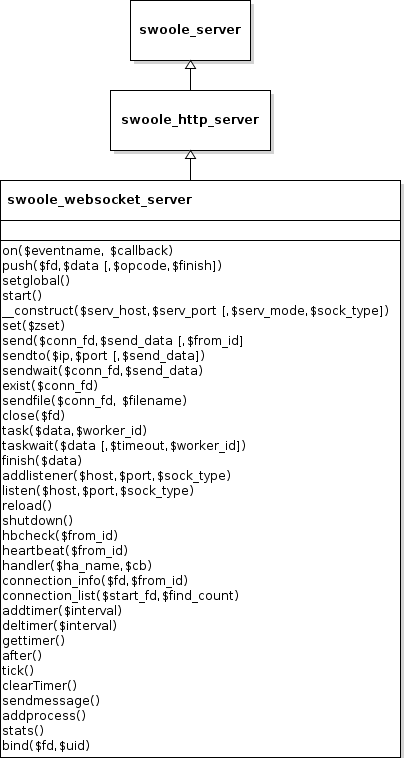
\includegraphics[scale=0.45]{class_swoole_websocket_server.png}
\caption{swoole\_websocket\_server类}
\end{figure}

\begin{compactitem}
\item \texttt{\$fd}:TCP连接的文件描述符(file description),在swoole\_server中是客户端的唯一标识符。
\item \texttt{\$from\_id}:来自于哪个reactor线程。
\item \texttt{\$conn\_fd}:网络字节序(long类型字段,IPv4的第4字节最小为1)。
\end{compactitem}


\begin{lstlisting}[language=PHP]

\end{lstlisting}


\section{WS Server}


\begin{lstlisting}[language=PHP]
<?php
/**
 * 创建WebSocket Server
 */
$wsserver = new swoole_websocket_server("127.0.0.1", 9502);

/**
 * 注册Server的事件回调函数open
 */
$wsserver->on('Open', function($server, $req) {
    echo "connection open: ".$req->fd;
});

/**
 * 注册Server的事件回调函数message
 */
$wsserver->on('Message', function($server, $frame) {
    echo "message: ".$frame->data;
    $server->push($frame->fd, json_encode(["hello", "world"]));
});

/**
 * 注册Server的事件回调函数close
 */
$wsserver->on('Close', function($server, $fd) {
    echo "connection close: ".$fd;
});

/**
 * 启动WebSocket Server
 */
$wsserver->start();
?>
\end{lstlisting}




\begin{lstlisting}[language=PHP]

\end{lstlisting}



\begin{lstlisting}[language=PHP]

\end{lstlisting}


\begin{lstlisting}[language=PHP]

\end{lstlisting}






\begin{lstlisting}[language=PHP]

\end{lstlisting}



\begin{lstlisting}[language=PHP]

\end{lstlisting}



\begin{lstlisting}[language=PHP]

\end{lstlisting}





\section{WSS Server}


\begin{lstlisting}[language=PHP]

\end{lstlisting}





\begin{lstlisting}[language=PHP]
<?php
$wssserver = new swoole_websocket_server("0.0.0.0",9527,SWOOLE_PROCESS,);
?>
\end{lstlisting}




\begin{lstlisting}[language=PHP]

\end{lstlisting}




\begin{lstlisting}[language=PHP]

\end{lstlisting}


\chapter{WebSocket Client}

\begin{lstlisting}[language=PHP]

\end{lstlisting}




\begin{lstlisting}[language=PHP]

\end{lstlisting}




\begin{lstlisting}[language=PHP]

\end{lstlisting}




\begin{lstlisting}[language=PHP]

\end{lstlisting}


\chapter{Async-IO}

\begin{lstlisting}[language=PHP]
$fp = stream_socket_client("tcp://127.0.0.1:80", $code, $msg, 3);
$http_request = "GET /index.html HTTP/1.1\r\n\r\n";
fwrite($fp, $http_request);
swoole_event_add($fp, function($fp){
    echo fread($fp, 8192);
    swoole_event_del($fp);
    fclose($fp);
});
swoole_timer_after(2000, function() {
    echo "2000ms timeout\n";
});
swoole_timer_tick(1000, function() {
    echo "1000ms interval\n";
});
\end{lstlisting}




\begin{lstlisting}[language=PHP]

\end{lstlisting}




\begin{lstlisting}[language=PHP]

\end{lstlisting}


\chapter{Task}


\begin{lstlisting}[language=PHP]
$serv = new swoole_server("127.0.0.1", 9502);
$serv->set(array('task_worker_num' => 4));
$serv->on('Receive', function($serv, $fd, $from_id, $data) {
    $task_id = $serv->task("Async");
    echo "Dispath AsyncTask: id=$task_id\n";
});
$serv->on('Task', function ($serv, $task_id, $from_id, $data) {
    echo "New AsyncTask[id=$task_id]".PHP_EOL;
    $serv->finish("$data -> OK");
});
$serv->on('Finish', function ($serv, $task_id, $data) {
    echo "AsyncTask[$task_id] Finish: $data".PHP_EOL;
});
$serv->start();
\end{lstlisting}




\begin{lstlisting}[language=PHP]

\end{lstlisting}






\begin{lstlisting}[language=PHP]

\end{lstlisting}




\begin{lstlisting}[language=PHP]

\end{lstlisting}




\begin{lstlisting}[language=PHP]

\end{lstlisting}




\begin{lstlisting}[language=PHP]

\end{lstlisting}




\begin{lstlisting}[language=PHP]

\end{lstlisting}




\begin{lstlisting}[language=PHP]

\end{lstlisting}




\begin{lstlisting}[language=PHP]

\end{lstlisting}




\begin{lstlisting}[language=PHP]

\end{lstlisting}




\begin{lstlisting}[language=PHP]

\end{lstlisting}




\begin{lstlisting}[language=PHP]

\end{lstlisting}





\begin{lstlisting}[language=PHP]

\end{lstlisting}




\begin{lstlisting}[language=PHP]

\end{lstlisting}




\begin{lstlisting}[language=PHP]

\end{lstlisting}




\begin{lstlisting}[language=PHP]

\end{lstlisting}




\begin{lstlisting}[language=PHP]

\end{lstlisting}




\begin{lstlisting}[language=PHP]

\end{lstlisting}




\begin{lstlisting}[language=PHP]

\end{lstlisting}




\begin{lstlisting}[language=PHP]

\end{lstlisting}




\begin{lstlisting}[language=PHP]

\end{lstlisting}




\begin{lstlisting}[language=PHP]

\end{lstlisting}




\begin{lstlisting}[language=PHP]

\end{lstlisting}




\begin{lstlisting}[language=PHP]

\end{lstlisting}





\begin{lstlisting}[language=PHP]

\end{lstlisting}




\begin{lstlisting}[language=PHP]

\end{lstlisting}



\begin{lstlisting}[language=PHP]

\end{lstlisting}




\begin{lstlisting}[language=PHP]

\end{lstlisting}




\begin{lstlisting}[language=PHP]

\end{lstlisting}




\begin{lstlisting}[language=PHP]

\end{lstlisting}




\begin{lstlisting}[language=PHP]

\end{lstlisting}




\begin{lstlisting}[language=PHP]

\end{lstlisting}




\begin{lstlisting}[language=PHP]

\end{lstlisting}




\begin{lstlisting}[language=PHP]

\end{lstlisting}





\begin{lstlisting}[language=PHP]

\end{lstlisting}




\begin{lstlisting}[language=PHP]

\end{lstlisting}




\begin{lstlisting}[language=PHP]

\end{lstlisting}




\begin{lstlisting}[language=PHP]

\end{lstlisting}




\begin{lstlisting}[language=PHP]

\end{lstlisting}




\begin{lstlisting}[language=PHP]

\end{lstlisting}




\begin{lstlisting}[language=PHP]

\end{lstlisting}




\begin{lstlisting}[language=PHP]

\end{lstlisting}




\begin{lstlisting}[language=PHP]

\end{lstlisting}




\begin{lstlisting}[language=PHP]

\end{lstlisting}




\begin{lstlisting}[language=PHP]

\end{lstlisting}




\begin{lstlisting}[language=PHP]

\end{lstlisting}




\begin{lstlisting}[language=PHP]

\end{lstlisting}




\begin{lstlisting}[language=PHP]

\end{lstlisting}





\begin{lstlisting}[language=PHP]

\end{lstlisting}




\begin{lstlisting}[language=PHP]

\end{lstlisting}







\begin{lstlisting}[language=PHP]

\end{lstlisting}





\begin{lstlisting}[language=PHP]

\end{lstlisting}



















\begin{lstlisting}[language=PHP]

\end{lstlisting}




\begin{lstlisting}[language=PHP]

\end{lstlisting}




\begin{lstlisting}[language=PHP]

\end{lstlisting}




\begin{lstlisting}[language=PHP]

\end{lstlisting}




\begin{lstlisting}[language=PHP]

\end{lstlisting}




\begin{lstlisting}[language=PHP]

\end{lstlisting}




\begin{lstlisting}[language=PHP]

\end{lstlisting}





\begin{lstlisting}[language=PHP]

\end{lstlisting}




\begin{lstlisting}[language=PHP]

\end{lstlisting}




\begin{lstlisting}[language=PHP]

\end{lstlisting}




\begin{lstlisting}[language=PHP]

\end{lstlisting}




\begin{lstlisting}[language=PHP]

\end{lstlisting}




\begin{lstlisting}[language=PHP]

\end{lstlisting}




\begin{lstlisting}[language=PHP]

\end{lstlisting}




\begin{lstlisting}[language=PHP]

\end{lstlisting}




\begin{lstlisting}[language=PHP]

\end{lstlisting}




\begin{lstlisting}[language=PHP]

\end{lstlisting}




\begin{lstlisting}[language=PHP]

\end{lstlisting}




\begin{lstlisting}[language=PHP]

\end{lstlisting}




\begin{lstlisting}[language=PHP]

\end{lstlisting}




\begin{lstlisting}[language=PHP]

\end{lstlisting}





\begin{lstlisting}[language=PHP]

\end{lstlisting}




\begin{lstlisting}[language=PHP]

\end{lstlisting}






\begin{lstlisting}[language=PHP]

\end{lstlisting}




\begin{lstlisting}[language=PHP]

\end{lstlisting}




\begin{lstlisting}[language=PHP]

\end{lstlisting}




\begin{lstlisting}[language=PHP]

\end{lstlisting}




\begin{lstlisting}[language=PHP]

\end{lstlisting}




\begin{lstlisting}[language=PHP]

\end{lstlisting}




\begin{lstlisting}[language=PHP]

\end{lstlisting}




\begin{lstlisting}[language=PHP]

\end{lstlisting}




\begin{lstlisting}[language=PHP]

\end{lstlisting}




\begin{lstlisting}[language=PHP]

\end{lstlisting}





\begin{lstlisting}[language=PHP]

\end{lstlisting}




\begin{lstlisting}[language=PHP]

\end{lstlisting}




\begin{lstlisting}[language=PHP]

\end{lstlisting}




\begin{lstlisting}[language=PHP]

\end{lstlisting}




\begin{lstlisting}[language=PHP]

\end{lstlisting}




\begin{lstlisting}[language=PHP]

\end{lstlisting}




\begin{lstlisting}[language=PHP]

\end{lstlisting}




\begin{lstlisting}[language=PHP]

\end{lstlisting}




\begin{lstlisting}[language=PHP]

\end{lstlisting}




\begin{lstlisting}[language=PHP]

\end{lstlisting}




\begin{lstlisting}[language=PHP]

\end{lstlisting}




\begin{lstlisting}[language=PHP]

\end{lstlisting}





\begin{lstlisting}[language=PHP]

\end{lstlisting}




\begin{lstlisting}[language=PHP]

\end{lstlisting}



\begin{lstlisting}[language=PHP]

\end{lstlisting}




\begin{lstlisting}[language=PHP]

\end{lstlisting}




\begin{lstlisting}[language=PHP]

\end{lstlisting}




\begin{lstlisting}[language=PHP]

\end{lstlisting}




\begin{lstlisting}[language=PHP]

\end{lstlisting}




\begin{lstlisting}[language=PHP]

\end{lstlisting}




\begin{lstlisting}[language=PHP]

\end{lstlisting}




\begin{lstlisting}[language=PHP]

\end{lstlisting}





\begin{lstlisting}[language=PHP]

\end{lstlisting}




\begin{lstlisting}[language=PHP]

\end{lstlisting}




\begin{lstlisting}[language=PHP]

\end{lstlisting}




\begin{lstlisting}[language=PHP]

\end{lstlisting}




\begin{lstlisting}[language=PHP]

\end{lstlisting}




\begin{lstlisting}[language=PHP]

\end{lstlisting}




\begin{lstlisting}[language=PHP]

\end{lstlisting}




\begin{lstlisting}[language=PHP]

\end{lstlisting}




\begin{lstlisting}[language=PHP]

\end{lstlisting}




\begin{lstlisting}[language=PHP]

\end{lstlisting}




\begin{lstlisting}[language=PHP]

\end{lstlisting}




\begin{lstlisting}[language=PHP]

\end{lstlisting}




\begin{lstlisting}[language=PHP]

\end{lstlisting}




\begin{lstlisting}[language=PHP]

\end{lstlisting}





\begin{lstlisting}[language=PHP]

\end{lstlisting}




\begin{lstlisting}[language=PHP]

\end{lstlisting}







\begin{lstlisting}[language=PHP]

\end{lstlisting}





\begin{lstlisting}[language=PHP]

\end{lstlisting}



















\begin{lstlisting}[language=PHP]

\end{lstlisting}




\begin{lstlisting}[language=PHP]

\end{lstlisting}




\begin{lstlisting}[language=PHP]

\end{lstlisting}




\begin{lstlisting}[language=PHP]

\end{lstlisting}




\begin{lstlisting}[language=PHP]

\end{lstlisting}




\begin{lstlisting}[language=PHP]

\end{lstlisting}




\begin{lstlisting}[language=PHP]

\end{lstlisting}





\begin{lstlisting}[language=PHP]

\end{lstlisting}




\begin{lstlisting}[language=PHP]

\end{lstlisting}




\begin{lstlisting}[language=PHP]

\end{lstlisting}




\begin{lstlisting}[language=PHP]

\end{lstlisting}




\begin{lstlisting}[language=PHP]

\end{lstlisting}




\begin{lstlisting}[language=PHP]

\end{lstlisting}




\begin{lstlisting}[language=PHP]

\end{lstlisting}




\begin{lstlisting}[language=PHP]

\end{lstlisting}




\begin{lstlisting}[language=PHP]

\end{lstlisting}




\begin{lstlisting}[language=PHP]

\end{lstlisting}




\begin{lstlisting}[language=PHP]

\end{lstlisting}




\begin{lstlisting}[language=PHP]

\end{lstlisting}




\begin{lstlisting}[language=PHP]

\end{lstlisting}




\begin{lstlisting}[language=PHP]

\end{lstlisting}





\begin{lstlisting}[language=PHP]

\end{lstlisting}




\begin{lstlisting}[language=PHP]

\end{lstlisting}






\begin{lstlisting}[language=PHP]

\end{lstlisting}




\begin{lstlisting}[language=PHP]

\end{lstlisting}




\begin{lstlisting}[language=PHP]

\end{lstlisting}




\begin{lstlisting}[language=PHP]

\end{lstlisting}




\begin{lstlisting}[language=PHP]

\end{lstlisting}




\begin{lstlisting}[language=PHP]

\end{lstlisting}




\begin{lstlisting}[language=PHP]

\end{lstlisting}




\begin{lstlisting}[language=PHP]

\end{lstlisting}




\begin{lstlisting}[language=PHP]

\end{lstlisting}




\begin{lstlisting}[language=PHP]

\end{lstlisting}





\begin{lstlisting}[language=PHP]

\end{lstlisting}




\begin{lstlisting}[language=PHP]

\end{lstlisting}




\begin{lstlisting}[language=PHP]

\end{lstlisting}




\begin{lstlisting}[language=PHP]

\end{lstlisting}




\begin{lstlisting}[language=PHP]

\end{lstlisting}




\begin{lstlisting}[language=PHP]

\end{lstlisting}




\begin{lstlisting}[language=PHP]

\end{lstlisting}




\begin{lstlisting}[language=PHP]

\end{lstlisting}




\begin{lstlisting}[language=PHP]

\end{lstlisting}




\begin{lstlisting}[language=PHP]

\end{lstlisting}




\begin{lstlisting}[language=PHP]

\end{lstlisting}




\begin{lstlisting}[language=PHP]

\end{lstlisting}





\begin{lstlisting}[language=PHP]

\end{lstlisting}




\begin{lstlisting}[language=PHP]

\end{lstlisting}



\begin{lstlisting}[language=PHP]

\end{lstlisting}




\begin{lstlisting}[language=PHP]

\end{lstlisting}




\begin{lstlisting}[language=PHP]

\end{lstlisting}




\begin{lstlisting}[language=PHP]

\end{lstlisting}




\begin{lstlisting}[language=PHP]

\end{lstlisting}




\begin{lstlisting}[language=PHP]

\end{lstlisting}




\begin{lstlisting}[language=PHP]

\end{lstlisting}




\begin{lstlisting}[language=PHP]

\end{lstlisting}





\begin{lstlisting}[language=PHP]

\end{lstlisting}




\begin{lstlisting}[language=PHP]

\end{lstlisting}




\begin{lstlisting}[language=PHP]

\end{lstlisting}




\begin{lstlisting}[language=PHP]

\end{lstlisting}




\begin{lstlisting}[language=PHP]

\end{lstlisting}




\begin{lstlisting}[language=PHP]

\end{lstlisting}




\begin{lstlisting}[language=PHP]

\end{lstlisting}




\begin{lstlisting}[language=PHP]

\end{lstlisting}




\begin{lstlisting}[language=PHP]

\end{lstlisting}




\begin{lstlisting}[language=PHP]

\end{lstlisting}




\begin{lstlisting}[language=PHP]

\end{lstlisting}




\begin{lstlisting}[language=PHP]

\end{lstlisting}




\begin{lstlisting}[language=PHP]

\end{lstlisting}




\begin{lstlisting}[language=PHP]

\end{lstlisting}





\begin{lstlisting}[language=PHP]

\end{lstlisting}




\begin{lstlisting}[language=PHP]

\end{lstlisting}








\begin{lstlisting}[language=PHP]

\end{lstlisting}





\begin{lstlisting}[language=PHP]

\end{lstlisting}



















\begin{lstlisting}[language=PHP]

\end{lstlisting}




\begin{lstlisting}[language=PHP]

\end{lstlisting}




\begin{lstlisting}[language=PHP]

\end{lstlisting}




\begin{lstlisting}[language=PHP]

\end{lstlisting}




\begin{lstlisting}[language=PHP]

\end{lstlisting}




\begin{lstlisting}[language=PHP]

\end{lstlisting}




\begin{lstlisting}[language=PHP]

\end{lstlisting}





\begin{lstlisting}[language=PHP]

\end{lstlisting}




\begin{lstlisting}[language=PHP]

\end{lstlisting}




\begin{lstlisting}[language=PHP]

\end{lstlisting}




\begin{lstlisting}[language=PHP]

\end{lstlisting}




\begin{lstlisting}[language=PHP]

\end{lstlisting}




\begin{lstlisting}[language=PHP]

\end{lstlisting}




\begin{lstlisting}[language=PHP]

\end{lstlisting}




\begin{lstlisting}[language=PHP]

\end{lstlisting}




\begin{lstlisting}[language=PHP]

\end{lstlisting}




\begin{lstlisting}[language=PHP]

\end{lstlisting}




\begin{lstlisting}[language=PHP]

\end{lstlisting}




\begin{lstlisting}[language=PHP]

\end{lstlisting}




\begin{lstlisting}[language=PHP]

\end{lstlisting}




\begin{lstlisting}[language=PHP]

\end{lstlisting}





\begin{lstlisting}[language=PHP]

\end{lstlisting}




\begin{lstlisting}[language=PHP]

\end{lstlisting}






\begin{lstlisting}[language=PHP]

\end{lstlisting}




\begin{lstlisting}[language=PHP]

\end{lstlisting}




\begin{lstlisting}[language=PHP]

\end{lstlisting}




\begin{lstlisting}[language=PHP]

\end{lstlisting}




\begin{lstlisting}[language=PHP]

\end{lstlisting}




\begin{lstlisting}[language=PHP]

\end{lstlisting}




\begin{lstlisting}[language=PHP]

\end{lstlisting}




\begin{lstlisting}[language=PHP]

\end{lstlisting}




\begin{lstlisting}[language=PHP]

\end{lstlisting}




\begin{lstlisting}[language=PHP]

\end{lstlisting}





\begin{lstlisting}[language=PHP]

\end{lstlisting}




\begin{lstlisting}[language=PHP]

\end{lstlisting}




\begin{lstlisting}[language=PHP]

\end{lstlisting}




\begin{lstlisting}[language=PHP]

\end{lstlisting}




\begin{lstlisting}[language=PHP]

\end{lstlisting}




\begin{lstlisting}[language=PHP]

\end{lstlisting}




\begin{lstlisting}[language=PHP]

\end{lstlisting}




\begin{lstlisting}[language=PHP]

\end{lstlisting}




\begin{lstlisting}[language=PHP]

\end{lstlisting}




\begin{lstlisting}[language=PHP]

\end{lstlisting}




\begin{lstlisting}[language=PHP]

\end{lstlisting}




\begin{lstlisting}[language=PHP]

\end{lstlisting}





\begin{lstlisting}[language=PHP]

\end{lstlisting}




\begin{lstlisting}[language=PHP]

\end{lstlisting}



\begin{lstlisting}[language=PHP]

\end{lstlisting}




\begin{lstlisting}[language=PHP]

\end{lstlisting}




\begin{lstlisting}[language=PHP]

\end{lstlisting}




\begin{lstlisting}[language=PHP]

\end{lstlisting}




\begin{lstlisting}[language=PHP]

\end{lstlisting}




\begin{lstlisting}[language=PHP]

\end{lstlisting}




\begin{lstlisting}[language=PHP]

\end{lstlisting}




\begin{lstlisting}[language=PHP]

\end{lstlisting}





\begin{lstlisting}[language=PHP]

\end{lstlisting}




\begin{lstlisting}[language=PHP]

\end{lstlisting}




\begin{lstlisting}[language=PHP]

\end{lstlisting}




\begin{lstlisting}[language=PHP]

\end{lstlisting}




\begin{lstlisting}[language=PHP]

\end{lstlisting}




\begin{lstlisting}[language=PHP]

\end{lstlisting}




\begin{lstlisting}[language=PHP]

\end{lstlisting}




\begin{lstlisting}[language=PHP]

\end{lstlisting}




\begin{lstlisting}[language=PHP]

\end{lstlisting}




\begin{lstlisting}[language=PHP]

\end{lstlisting}




\begin{lstlisting}[language=PHP]

\end{lstlisting}




\begin{lstlisting}[language=PHP]

\end{lstlisting}




\begin{lstlisting}[language=PHP]

\end{lstlisting}




\begin{lstlisting}[language=PHP]

\end{lstlisting}





\begin{lstlisting}[language=PHP]

\end{lstlisting}




\begin{lstlisting}[language=PHP]

\end{lstlisting}








\begin{lstlisting}[language=PHP]

\end{lstlisting}





\begin{lstlisting}[language=PHP]

\end{lstlisting}



















\begin{lstlisting}[language=PHP]

\end{lstlisting}




\begin{lstlisting}[language=PHP]

\end{lstlisting}




\begin{lstlisting}[language=PHP]

\end{lstlisting}




\begin{lstlisting}[language=PHP]

\end{lstlisting}




\begin{lstlisting}[language=PHP]

\end{lstlisting}




\begin{lstlisting}[language=PHP]

\end{lstlisting}




\begin{lstlisting}[language=PHP]

\end{lstlisting}





\begin{lstlisting}[language=PHP]

\end{lstlisting}




\begin{lstlisting}[language=PHP]

\end{lstlisting}




\begin{lstlisting}[language=PHP]

\end{lstlisting}




\begin{lstlisting}[language=PHP]

\end{lstlisting}




\begin{lstlisting}[language=PHP]

\end{lstlisting}




\begin{lstlisting}[language=PHP]

\end{lstlisting}




\begin{lstlisting}[language=PHP]

\end{lstlisting}




\begin{lstlisting}[language=PHP]

\end{lstlisting}




\begin{lstlisting}[language=PHP]

\end{lstlisting}




\begin{lstlisting}[language=PHP]

\end{lstlisting}




\begin{lstlisting}[language=PHP]

\end{lstlisting}




\begin{lstlisting}[language=PHP]

\end{lstlisting}




\begin{lstlisting}[language=PHP]

\end{lstlisting}




\begin{lstlisting}[language=PHP]

\end{lstlisting}





\begin{lstlisting}[language=PHP]

\end{lstlisting}




\begin{lstlisting}[language=PHP]

\end{lstlisting}






\begin{lstlisting}[language=PHP]

\end{lstlisting}




\begin{lstlisting}[language=PHP]

\end{lstlisting}




\begin{lstlisting}[language=PHP]

\end{lstlisting}




\begin{lstlisting}[language=PHP]

\end{lstlisting}




\begin{lstlisting}[language=PHP]

\end{lstlisting}




\begin{lstlisting}[language=PHP]

\end{lstlisting}




\begin{lstlisting}[language=PHP]

\end{lstlisting}




\begin{lstlisting}[language=PHP]

\end{lstlisting}




\begin{lstlisting}[language=PHP]

\end{lstlisting}




\begin{lstlisting}[language=PHP]

\end{lstlisting}





\begin{lstlisting}[language=PHP]

\end{lstlisting}




\begin{lstlisting}[language=PHP]

\end{lstlisting}




\begin{lstlisting}[language=PHP]

\end{lstlisting}




\begin{lstlisting}[language=PHP]

\end{lstlisting}




\begin{lstlisting}[language=PHP]

\end{lstlisting}




\begin{lstlisting}[language=PHP]

\end{lstlisting}




\begin{lstlisting}[language=PHP]

\end{lstlisting}




\begin{lstlisting}[language=PHP]

\end{lstlisting}




\begin{lstlisting}[language=PHP]

\end{lstlisting}




\begin{lstlisting}[language=PHP]

\end{lstlisting}




\begin{lstlisting}[language=PHP]

\end{lstlisting}




\begin{lstlisting}[language=PHP]

\end{lstlisting}





\begin{lstlisting}[language=PHP]

\end{lstlisting}




\begin{lstlisting}[language=PHP]

\end{lstlisting}



\begin{lstlisting}[language=PHP]

\end{lstlisting}




\begin{lstlisting}[language=PHP]

\end{lstlisting}




\begin{lstlisting}[language=PHP]

\end{lstlisting}




\begin{lstlisting}[language=PHP]

\end{lstlisting}




\begin{lstlisting}[language=PHP]

\end{lstlisting}




\begin{lstlisting}[language=PHP]

\end{lstlisting}




\begin{lstlisting}[language=PHP]

\end{lstlisting}




\begin{lstlisting}[language=PHP]

\end{lstlisting}





\begin{lstlisting}[language=PHP]

\end{lstlisting}




\begin{lstlisting}[language=PHP]

\end{lstlisting}




\begin{lstlisting}[language=PHP]

\end{lstlisting}




\begin{lstlisting}[language=PHP]

\end{lstlisting}




\begin{lstlisting}[language=PHP]

\end{lstlisting}




\begin{lstlisting}[language=PHP]

\end{lstlisting}




\begin{lstlisting}[language=PHP]

\end{lstlisting}




\begin{lstlisting}[language=PHP]

\end{lstlisting}




\begin{lstlisting}[language=PHP]

\end{lstlisting}




\begin{lstlisting}[language=PHP]

\end{lstlisting}




\begin{lstlisting}[language=PHP]

\end{lstlisting}




\begin{lstlisting}[language=PHP]

\end{lstlisting}




\begin{lstlisting}[language=PHP]

\end{lstlisting}




\begin{lstlisting}[language=PHP]

\end{lstlisting}





\begin{lstlisting}[language=PHP]

\end{lstlisting}




\begin{lstlisting}[language=PHP]

\end{lstlisting}







\begin{lstlisting}[language=PHP]

\end{lstlisting}





\begin{lstlisting}[language=PHP]

\end{lstlisting}



















\begin{lstlisting}[language=PHP]

\end{lstlisting}




\begin{lstlisting}[language=PHP]

\end{lstlisting}




\begin{lstlisting}[language=PHP]

\end{lstlisting}




\begin{lstlisting}[language=PHP]

\end{lstlisting}




\begin{lstlisting}[language=PHP]

\end{lstlisting}




\begin{lstlisting}[language=PHP]

\end{lstlisting}




\begin{lstlisting}[language=PHP]

\end{lstlisting}





\begin{lstlisting}[language=PHP]

\end{lstlisting}




\begin{lstlisting}[language=PHP]

\end{lstlisting}




\begin{lstlisting}[language=PHP]

\end{lstlisting}




\begin{lstlisting}[language=PHP]

\end{lstlisting}




\begin{lstlisting}[language=PHP]

\end{lstlisting}




\begin{lstlisting}[language=PHP]

\end{lstlisting}




\begin{lstlisting}[language=PHP]

\end{lstlisting}




\begin{lstlisting}[language=PHP]

\end{lstlisting}




\begin{lstlisting}[language=PHP]

\end{lstlisting}




\begin{lstlisting}[language=PHP]

\end{lstlisting}




\begin{lstlisting}[language=PHP]

\end{lstlisting}




\begin{lstlisting}[language=PHP]

\end{lstlisting}




\begin{lstlisting}[language=PHP]

\end{lstlisting}




\begin{lstlisting}[language=PHP]

\end{lstlisting}





\begin{lstlisting}[language=PHP]

\end{lstlisting}




\begin{lstlisting}[language=PHP]

\end{lstlisting}






\begin{lstlisting}[language=PHP]

\end{lstlisting}




\begin{lstlisting}[language=PHP]

\end{lstlisting}




\begin{lstlisting}[language=PHP]

\end{lstlisting}




\begin{lstlisting}[language=PHP]

\end{lstlisting}




\begin{lstlisting}[language=PHP]

\end{lstlisting}




\begin{lstlisting}[language=PHP]

\end{lstlisting}




\begin{lstlisting}[language=PHP]

\end{lstlisting}




\begin{lstlisting}[language=PHP]

\end{lstlisting}




\begin{lstlisting}[language=PHP]

\end{lstlisting}




\begin{lstlisting}[language=PHP]

\end{lstlisting}





\begin{lstlisting}[language=PHP]

\end{lstlisting}




\begin{lstlisting}[language=PHP]

\end{lstlisting}




\begin{lstlisting}[language=PHP]

\end{lstlisting}




\begin{lstlisting}[language=PHP]

\end{lstlisting}




\begin{lstlisting}[language=PHP]

\end{lstlisting}




\begin{lstlisting}[language=PHP]

\end{lstlisting}




\begin{lstlisting}[language=PHP]

\end{lstlisting}




\begin{lstlisting}[language=PHP]

\end{lstlisting}




\begin{lstlisting}[language=PHP]

\end{lstlisting}




\begin{lstlisting}[language=PHP]

\end{lstlisting}




\begin{lstlisting}[language=PHP]

\end{lstlisting}




\begin{lstlisting}[language=PHP]

\end{lstlisting}





\begin{lstlisting}[language=PHP]

\end{lstlisting}




\begin{lstlisting}[language=PHP]

\end{lstlisting}



\begin{lstlisting}[language=PHP]

\end{lstlisting}




\begin{lstlisting}[language=PHP]

\end{lstlisting}




\begin{lstlisting}[language=PHP]

\end{lstlisting}




\begin{lstlisting}[language=PHP]

\end{lstlisting}




\begin{lstlisting}[language=PHP]

\end{lstlisting}




\begin{lstlisting}[language=PHP]

\end{lstlisting}




\begin{lstlisting}[language=PHP]

\end{lstlisting}




\begin{lstlisting}[language=PHP]

\end{lstlisting}





\begin{lstlisting}[language=PHP]

\end{lstlisting}




\begin{lstlisting}[language=PHP]

\end{lstlisting}




\begin{lstlisting}[language=PHP]

\end{lstlisting}




\begin{lstlisting}[language=PHP]

\end{lstlisting}




\begin{lstlisting}[language=PHP]

\end{lstlisting}




\begin{lstlisting}[language=PHP]

\end{lstlisting}




\begin{lstlisting}[language=PHP]

\end{lstlisting}




\begin{lstlisting}[language=PHP]

\end{lstlisting}




\begin{lstlisting}[language=PHP]

\end{lstlisting}




\begin{lstlisting}[language=PHP]

\end{lstlisting}




\begin{lstlisting}[language=PHP]

\end{lstlisting}




\begin{lstlisting}[language=PHP]

\end{lstlisting}




\begin{lstlisting}[language=PHP]

\end{lstlisting}




\begin{lstlisting}[language=PHP]

\end{lstlisting}





\begin{lstlisting}[language=PHP]

\end{lstlisting}




\begin{lstlisting}[language=PHP]

\end{lstlisting}

